\section{Example: Losev-Manin Space}
\label{sec:losev-manin-space}
    Now let us see an example of $\calm_{0, w}$ 
	with the weight vector $w = \{1, 1, \epsilon, \epsilon, \epsilon\}$,
    each entry denoted by 1, 2, 3, 4 and 5.
	In general this type of space is called \textbf{Losev-Manin Space}
	From definition the reduced weight graph of the weight vector $w = \{1, 1, \epsilon, \epsilon, \epsilon\}$ is as in Figure \ref{fig:losev-manin5-reduced-graph}.
    
    \begin{figure}
	\begin{center}
	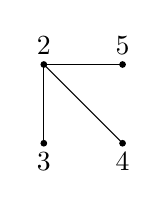
\begin{tikzpicture}
		\draw[black, thin] (0, 1) -- (1, 1);
		\draw[black, thin] (0, 0) -- (0, 1);
		\draw[black, thin] (0, 1) -- (1, 0);
		\filldraw[black] (1,0) circle (1pt) node[anchor=north] {$4$};
		\filldraw[black] (0,0) circle (1pt) node[anchor=north] {$3$};
		\filldraw[black] (0,1) circle (1pt) node[anchor=south] {$2$};
		\filldraw[black] (1,1) circle (1pt) node[anchor=south] {$5$};
	\end{tikzpicture}
	\end{center}
	\caption{The reduced weight graph $G$ of the weight vector $w = \{1, 1, \epsilon, \epsilon, \epsilon\}$.}
	\label{fig:losev-manin5-reduced-graph}
    \end{figure}
    
    Then in order to construct fan,
    we consider the building set of $1$-connected flats,
    whose definition we can recall from Subsection \ref{subsec:graphic-building-set}.
    From the reduced weight graph above, we see that the flats in the graphs are
    \begin{center}
		\begin{tabular}{ |c|c|c|c|} 
		\hline
 		Rank 1 & $F_1$ & $F_2$ & $F_3$  \\ \hline
 		& 
		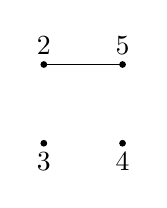
\begin{tikzpicture}
		\draw[black, thin] (0, 1) -- (1, 1);
		\filldraw[black] (1,0) circle (1pt) node[anchor=north] {$4$};
		\filldraw[black] (0,0) circle (1pt) node[anchor=north] {$3$};
		\filldraw[black] (0,1) circle (1pt) node[anchor=south] {$2$};
		\filldraw[black] (1,1) circle (1pt) node[anchor=south] {$5$};
		\end{tikzpicture}
		& 
		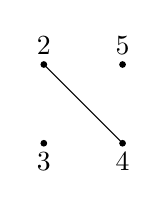
\begin{tikzpicture}
		\draw[black, thin] (0, 1) -- (1, 0);
		\filldraw[black] (1,0) circle (1pt) node[anchor=north] {$4$};
		\filldraw[black] (0,0) circle (1pt) node[anchor=north] {$3$};
		\filldraw[black] (0,1) circle (1pt) node[anchor=south] {$2$};
		\filldraw[black] (1,1) circle (1pt) node[anchor=south] {$5$};
		\end{tikzpicture}
		& 
		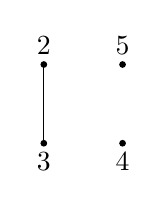
\begin{tikzpicture}
		\draw[black, thin] (0, 1) -- (0, 0);
		\filldraw[black] (1,0) circle (1pt) node[anchor=north] {$4$};
		\filldraw[black] (0,0) circle (1pt) node[anchor=north] {$3$};
		\filldraw[black] (0,1) circle (1pt) node[anchor=south] {$2$};
		\filldraw[black] (1,1) circle (1pt) node[anchor=south] {$5$};
		\end{tikzpicture}
		\\
		\hline
 		Rank 2 & $F_4$ & $F_5$ & $F_6$ \\ \hline
 		& 
		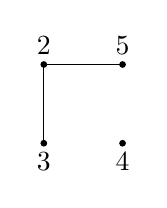
\begin{tikzpicture}
		\draw[black, thin] (0, 1) -- (1, 1);
		\draw[black, thin] (0, 1) -- (0, 0);
		\filldraw[black] (1,0) circle (1pt) node[anchor=north] {$4$};
		\filldraw[black] (0,0) circle (1pt) node[anchor=north] {$3$};
		\filldraw[black] (0,1) circle (1pt) node[anchor=south] {$2$};
		\filldraw[black] (1,1) circle (1pt) node[anchor=south] {$5$};
		\end{tikzpicture}
		& 
		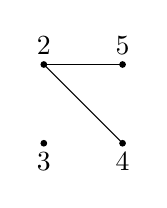
\begin{tikzpicture}
		\draw[black, thin] (0, 1) -- (1, 1);
		\draw[black, thin] (0, 1) -- (1, 0);
		\filldraw[black] (1,0) circle (1pt) node[anchor=north] {$4$};
		\filldraw[black] (0,0) circle (1pt) node[anchor=north] {$3$};
		\filldraw[black] (0,1) circle (1pt) node[anchor=south] {$2$};
		\filldraw[black] (1,1) circle (1pt) node[anchor=south] {$5$};
		\end{tikzpicture}
		& 
		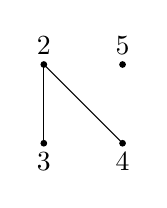
\begin{tikzpicture}
		\draw[black, thin] (0, 1) -- (0, 0);
		\draw[black, thin] (0, 1) -- (1, 0);
		\filldraw[black] (1,0) circle (1pt) node[anchor=north] {$4$};
		\filldraw[black] (0,0) circle (1pt) node[anchor=north] {$3$};
		\filldraw[black] (0,1) circle (1pt) node[anchor=south] {$2$};
		\filldraw[black] (1,1) circle (1pt) node[anchor=south] {$5$};
		\end{tikzpicture}
		\\
		\hline
		\end{tabular}
	\captionof{table}{The $1$-connected flats of $G((1, 1, \epsilon, \epsilon, \epsilon))$.} 
    \end{center}
    Reading off the projection from the graph $G$ as a subgraph of the complete graph on $4$ vertices
    we obtain a list of vectors that give us a combinatorial interpretation of $B'(G)$. 
    The list of projections are obtained as follows:
    \begin{align*}
    \pr_w(v_{1, 2}) = \pr_w(v_{3, 4}) = \pr_w(v_{4, 5}) = \varnothing \\
    \pr_w(v_{1, 3}) = \pr_w(v_{2, 5}) = \pr_w(v_{2, 4}) = V_{F_5} \\
    \pr_w(v_{1, 4}) = \pr_w(v_{2, 5}) = \pr_w(v_{2, 3}) = V_{F_6} \\
    \pr_w(v_{1, 5}) = \pr_w(v_{2, 4}) = \pr_w(v_{2, 3}) = V_{F_4} \\
    \pr_w(v_{2, 3}) = V_{F_3} \\
    \pr_w(v_{2, 4}) = V_{F_2} \\
    \pr_w(v_{2, 5}) = V_{F_1} \\
    \end{align*}
    Since the corresponding flat of each $V_{F_i}$ indicates who the nodes are connected in the phylogenetic trees, 
    by gluing cones defined by phylogenetic trees, 
    we obtain a combinatorial interpretation of the Bergman fan as follows:
    
    \begin{figure}
	\begin{center}
	\begin{tikzpicture}
	    % Draw fan skeleton
		\draw[black, thin] (0, 0) -- (4, 0);
		\draw[black, thin] (0, 0) -- (0, 4);
		\draw[black, thin] (0, 0) -- (0, -4);
		\draw[black, thin] (0, 0) -- (-4, 0);
		\draw[black, thin] (0, 0) -- (4, 4);
		\draw[black, thin] (0, 0) -- (-4, -4);
		\filldraw[black] (4, 0) circle (1pt) node[anchor=south] {$V_{F_5}$};
		\filldraw[black] (4, 4) circle (1pt) node[anchor=south] {$V_{F_1}$};
		\filldraw[black] (0, 4) circle (1pt) node[anchor=south] {$V_{F_4}$};
		\filldraw[black] (0, -4) circle (1pt) node[anchor=north] {$V_{F_2}$};
		\filldraw[black] (-4, -4) circle (1pt) node[anchor=north] {$V_{F_6}$};
		\filldraw[black] (-4, 0) circle (1pt) node[anchor=south] {$V_{F_3}$};
		
		
		% Draw labelled trees 
		% First quadrant
		% Lower
 		\draw (2.6, 2) node[above]{ \tiny 1}-- (4.2, 2) node[above]{\tiny 2};
		\draw (3.0, 2)-- (3.0, 1) node[below]{\tiny 3};
 		\draw (3.4, 2)-- (3.4, 1) node[below]{\tiny 4};
 		\draw (3.8, 2)-- (3.8, 1) node[below]{\tiny 5};

		% Upper
		 \draw (1.0, 4) node[above]{ \tiny 1}-- (2.6, 4) node[above]{\tiny 2};
		\draw (1.4, 4)-- (1.4, 3) node[below]{\tiny 5};
 		\draw (1.8, 4)-- (1.8, 3) node[below]{\tiny 3};
 		\draw (2.2, 4)-- (2.2, 3) node[below]{\tiny 4};
		
		% Second quadrant
		% Lower
		 \draw (-3.4, 2.6) node[above]{ \tiny 1}-- (-1.8, 2.6) node[above]{\tiny 2};
		\draw (-2.2, 2.6)-- (-2.2, 1.6) node[below]{\tiny 3};
 		\draw (-2.6, 2.6)-- (-2.6, 1.6) node[below]{\tiny 5};
 		\draw (-3.0, 2.6)-- (-3.0, 1.6) node[below]{\tiny 4};
		
		% Third quadrant
		% Lower
		\draw (-2.4, -3.0) node[above]{ \tiny 1}-- (-0.8, -3.0) node[above]{\tiny 2};
		\draw (-1.2, -3.0)-- (-1.2, -4.0) node[below]{\tiny 3};
 		\draw (-1.6, -3.0)-- (-1.6, -4.0) node[below]{\tiny 4};
 		\draw (-2.0, -3.0)-- (-2.0, -4.0) node[below]{\tiny 5};
		
		% Upper
		\draw (-4.2, -1.0) node[above]{ \tiny 1}-- (-2.6, -1.0) node[above]{\tiny 2};
		\draw (-3.0, -1.0)-- (-3.0, -2.0) node[below]{\tiny 4};
 		\draw (-3.4, -1.0)-- (-3.4, -2.0) node[below]{\tiny 3};
 		\draw (-3.8, -1.0)-- (-3.8, -2.0) node[below]{\tiny 5};
		
		% Fourth quadrant
		% Lower
		\draw (1.4, -2.0) node[above]{ \tiny 1}-- (3.0, -2.0) node[above]{\tiny 2};
		\draw (2.6, -2.0)-- (2.6, -3.0) node[below]{\tiny 4};
 		\draw (2.2, -2.0)-- (2.2, -3.0) node[below]{\tiny 5};
 		\draw (1.8, -2.0)-- (1.8, -3.0) node[below]{\tiny 3};
		
	\end{tikzpicture}
	\end{center}
	\caption{The combinatorial description of the Bergman fan,
	with each $2$-dimensional cone corresponding to a combinatorial type of the phylogenetic tree -- a type of curve.
	The primitive generators of the one dimensional cones of the fan are $V_{F_{i}}$ for $i \in [6]$. 
	They are vectors $(1, 0), (1, 1), (0,1), (-1, 0), (-1, -1), (0, -1)$ 
	on a plane.}
    \end{figure}
    
    To calculate the cohomology ring of the $\overline{M}_{0, 5}$,
    we first define lattice of flats, which is defined as following:
    \begin{definition}[Lattice of flats]
        A poset of closed subsets of a matroid.    
    \end{definition}
    
    In this example, the building set $\mathcal{G}$ is the set of all flats.
    Then Chow ring $A^\ast(X_{\Sigma_G})$ is the quotient of $\Z[x_\sigma: \sigma \in \mathcal{G}]$ 
    mod out the ideal $SR(\Sigma_\mathcal{G}) + L_{\Sigma_{\mathcal{G}}}$
    where $SR(\Sigma_\mathcal{G})$ is a set of products of rays $v_{F_i}$ that do not form a cone. 
    To calculate the Chow ring, which is equivalent to the cohomology ring in this case, 
    we have 
    \begin{align*}
    	A^\ast(X_{\Sigma_\mathcal{G}}) &= \frac{\Z[x_1, x_2, x_3, x_4, x_5, x_6]}{I_1}\\
	&\cong \frac{\Z[x, y, z, w]}{\langle x^3, y^3, z^3, w^3, x^2 + y^2, x^2 + z^2, x^2 + w^2, xy, xz, xw \rangle}.
    \end{align*}
    where $I = \langle x_1x_2, x_1x_3, x_1x_4, x_2x_3, x_2x_6, x_3x_5, x_4x_5, x_5x_6, x_4x_6, x_1 + x_5 - x_3 - x_4, x_1 + x_6 - x_2 - x_4, x_3 + x_6 - x_2 - x_5 \rangle$.
    The mod-out ideal $I$ can be calculated by calculating 
    the two equivalence relations in previous chapter on Chow ring as follows.
    \begin{enumerate}
    \item[(1)]
	Notice that $V_{F_1}$ can only forms cones with $V_{F_4}$ and $V_{F_5}$;
	$V_{F_2}$ only forms cones with $V_{F_5}$ and $V_{F_6}$;
	$V_{F_3}$ only forms cones with $V_{F_4}$ and $V_{F_6}$;
	$V_{F_4}$ only forms cones with $V_{F_1}$ and $V_{F_3}$;
	$V_{F_5}$ only forms cones with $V_{F_1}$ and $V_{F_2}$;
	$V_{F_6}$ only forms cones with $V_{F_2}$ and $V_{F_3}$.
	We thus set the complimentary product of set of $D_i$'s to zero,
	obtaining
	\begin{align*}
		D_1 D_2 &= D_1 D_3 = D_1 D_6 = 0 \\
		D_2 D_1 &= D_2 D_3 = D_2 D_4 = 0 \\
		D_3 D_1 &= D_3 D_2 = D_3 D_5 = 0 \\
		D_4 D_2 &= D_4 D_5 = D_4 D_6 = 0 \\
		D_5 D_3 &= D_5 D_4 = D_5 D_6 = 0 \\
		D_6 D_1 &= D_6 D_4 = D_6 D_5 = 0 \\
	\end{align*}
	Deleting repetitive information because of commutativity,
	we have 
	\begin{align*}
		D_1 D_2 &= 0 \\
		D_1 D_3 &= 0 \\
		D_1 D_6 &= 0 \\
		D_2 D_3 &= 0 \\
		D_2 D_4 &= 0 \\
		D_3 D_5 &= 0 \\
		D_4 D_5 &= 0 \\
		D_4 D_6 &= 0 \\
		D_5 D_6 &= 0 
 	\end{align*}
	Then pick a basis of this ambient $2$-dimensional 
	ambient vector space $\calb = \{V_{F_4}, V_{F_5}\}$.
	
	\item[(2)]
	For the second relationship,
	we take the sum of inner products of every generators with 
	each element in the basis as follows.
	For $V_{F_4}$ we have
	\[
		\sum\limits_{i=1}^6 \inner{V_{F_i}, V_{F_4}} D_i = 
		D_1 + D_4 - D_2 - D_6 = 0.
	\]
	For $V_{F_5}$ we have
	\[
		\sum\limits_{i=1}^6 \inner{V_{F_i}, V_{F_5}} D_i = 
		D_1 + D_5 - D_3 - D_6 = 0.
	\]
	These two equations give us
	\[
	D_1 + D_5 = D_3 + D_6, D_1 + D_4 = D_2 + D_6
	\]
    \end{enumerate}
    Using these two relations, renaming and canceling out some variables, 
    we obtain the desired cohomology of the Losiv-Manin space. 
    Other Losiv-Manin spaces with $l \ge 3$ will generate similar star-like Bergman combinatorial structures as well,
    for which we can calculate the toric variety and the Chow ring accordingly. 
    
    